%%%%%%%%%%%%%%%%%%%%%%%%%%%%%%%%%%%%%%%%%%%%%%%%%%%%%%%%%%%%%%%%%%%%%%%%%%%%
%% Author template for Operations Reseacrh (opre) for articles with no e-companion (EC)
%% Mirko Janc, Ph.D., INFORMS, mirko.janc@informs.org
%% ver. 0.95, December 2010
%%%%%%%%%%%%%%%%%%%%%%%%%%%%%%%%%%%%%%%%%%%%%%%%%%%%%%%%%%%%%%%%%%%%%%%%%%%%
%\documentclass[opre,blindrev]{informs3}
\documentclass[opre,nonblindrev]{informs3} % current default for manuscript submission

\SingleSpacedXI
\twocolumn

%\OneAndAHalfSpacedXII % Made default 4/4/2014 at request

%\OneAndAHalfSpacedXI % current default line spacing
%\OneAndAHalfSpacedXII
%\DoubleSpacedXII

% If hyperref is used, dvi-to-ps driver of choice must be declared as
%   an additional option to the \documentclass. For example
%\documentclass[dvips,opre]{informs3}      % if dvips is used
%\documentclass[dvipsone,opre]{informs3}   % if dvipsone is used, etc.

%%% OPRE uses endnotes. If you do not use them, put a percent sign before
%%% the \theendnotes command. This template does show how to use them.
\usepackage{endnotes}
\let\footnote=\endnote
\let\enotesize=\normalsize
\def\notesname{Endnotes}%
\def\makeenmark{$^{\theenmark}$}
\def\enoteformat{\rightskip0pt\leftskip0pt\parindent=1.75em
  \leavevmode\llap{\theenmark.\enskip}}

% Private macros here (check that there is no clash with the style)

% Natbib setup for author-year style
\usepackage{natbib}
 \bibpunct[, ]{(}{)}{,}{a}{}{,}%
 \def\bibfont{\small}%
 \def\bibsep{\smallskipamount}%
 \def\bibhang{24pt}%
 \def\newblock{\ }%
 \def\BIBand{and}%

%% Setup of theorem styles. Outcomment only one.
%% Preferred default is the first option.
\TheoremsNumberedThrough     % Preferred (Theorem 1, Lemma 1, Theorem 2)
%\TheoremsNumberedByChapter  % (Theorem 1.1, Lema 1.1, Theorem 1.2)
\ECRepeatTheorems

%% Setup of the equation numbering system. Outcomment only one.
%% Preferred default is the first option.
\EquationsNumberedThrough    % Default: (1), (2), ...
%\EquationsNumberedBySection % (1.1), (1.2), ...

% In the reviewing and copyediting stage enter the manuscript number.
%\MANUSCRIPTNO{} % When the article is logged in and DOI assigned to it,
                 %   this manuscript number is no longer necessary
                 
\usepackage{amsfonts}
\usepackage{color}
\usepackage{subeqnarray}
\usepackage{multirow}
\usepackage{amsmath}
\usepackage[english]{babel}       
\usepackage[ruled,vlined]{algorithm2e}
\usepackage{tikz}


%\textwidth=18.5 cm 




%%%%%%%%%%%%%%%%
\begin{document}
%%%%%%%%%%%%%%%%

\newcommand{\pdef}{\stackrel{\triangle}{=}}
\newcommand{\ds}{\displaystyle}
\newcommand{\ba}{\begin{array}}
	\newcommand{\ea}{\end{array}}
\newcommand{\conv}{\mbox{conv}}
\newcommand{\re}{\mathbb{R}}
\newcommand{\virg}{``}
\newcommand{\spa}{~}
\def\refe#1{(\ref{#1})}

% Outcomment only when entries are known. Otherwise leave as is and
%   default values will be used.
%\setcounter{page}{1}
%\VOLUME{00}%
%\NO{0}%
%\MONTH{Xxxxx}% (month or a similar seasonal id)
%\YEAR{0000}% e.g., 2005
%\FIRSTPAGE{000}%
%\LASTPAGE{000}%
%\SHORTYEAR{00}% shortened year (two-digit)
%\ISSUE{0000} %
%\LONGFIRSTPAGE{0001} %
%\DOI{10.1287/xxxx.0000.0000}%

% Author's names for the running heads
% Sample depending on the number of authors;
% \RUNAUTHOR{Jones}
% \RUNAUTHOR{Jones and Wilson}
% \RUNAUTHOR{Jones, Miller, and Wilson}
% \RUNAUTHOR{Jones et al.} % for four or more authors
% Enter authors following the given pattern:
\RUNAUTHOR{M. Avolio}

% Title or shortened title suitable for running heads. Sample:
% \RUNTITLE{Bundling Information Goods of Decreasing Value}
% Enter the (shortened) title:
\RUNTITLE{Balancing the average weighted completion times}

% Full title. Sample:
% \TITLE{Bundling Information Goods of Decreasing Value}
% Enter the full title:
\TITLE{Balancing the average weighted completion times in a scheduling problem with two classes of jobs: a genetic algorithm-based heuristics. }

% Block of authors and their affiliations starts here:
% NOTE: Authors with same affiliation, if the order of authors allows,
%   should be entered in ONE field, separated by a comma.
%   \EMAIL field can be repeated if more than one author
\ARTICLEAUTHORS{%
\AUTHOR{Matteo Avolio}
\AFF{Department of Mathematics and Computer Science, University of Calabria, Rende (CS), Italy, \EMAIL{matteo.avolio@unical.it}} %, \URL{}}
% Enter all authors
} % end of the block

\ABSTRACT{Balancing the average weighted completion times among two classes of jobs (BAWCT) could be interpreted as a cooperative multiagent scheduling problem. BAWCT was introduced in \cite{av-fud20} and it was explored in [2] where the authors proved its NP-hardness, providing a Lagrangian relaxation based approach for solving it heuristically. Since their approach requires to solve, at each iteration, a Linear Programming problem that it's not a very difficult task but however requires some computational time, in this work we propose a genetic algorithm-based heuristics to speed up the resolution process.\\
Numerical results are presented on the same datasets used in literature to empirically show the efficiency of the proposed approach. }
%

% Sample
%\KEYWORDS{deterministic inventory theory; infinite linear programming duality;
%  existence of optimal policies; semi-Markov decision process; cyclic schedule}

% Fill in data. If unknown, outcomment the field
\KEYWORDS{Scheduling; single-machine; multiagent; genetic algorithm} 
\HISTORY{}

\maketitle
%%%%%%%%%%%%%%%%%%%%%%%%%%%%%%%%%%%%%%%%%%%%%%%%%%%%%%%%%%%%%%%%%%%%%%

% Samples of sectioning (and labeling) in OPRE
% NOTE: (1) \section and \subsection do NOT end with a period
%       (2) \subsubsection and lower need end punctuation
%       (3) capitalization is as shown (title style).
%
%\section{Introduction.}\label{intro} %%1.
%\subsection{Duality and the Classical EOQ Problem.}\label{class-EOQ} %% 1.1.
%\subsection{Outline.}\label{outline1} %% 1.2.
%\subsubsection{Cyclic Schedules for the General Deterministic SMDP.}
%  \label{cyclic-schedules} %% 1.2.1
%\section{Problem Description.}\label{problemdescription} %% 2.

% Text of your paper here
\section{Introduction}
Allocating resources to tasks over given time periods with the aim of optimizing one or more objectives is what the theory of scheduling focus on. Scheduling, as a decision making process, plays a very important role in a lot of contexts such as manufacturing, production, transportation, and distribution (see as references \cite{pinedo09,pinedo16}). Unfortunately solving this kind of problems often is not easy and, however, it depends on the assumptions made on the problems themselves.\\
In the first years of the century, with publication of \cite{agnetis04} and \cite{baker2003}, a new scheduling model was introduced to take into account the presence of two or more agents. In multiagent scheduling problems (see \cite{agnetis-book14}) each agent has its own set of tasks to be processed and its own objective function to be optimized. The difficulty of this kind of problems arises from the fact that the agents share the processing resources.\\
\cite{baker2003}, in a multiagent context, faces the problem of minimizing three different objective functions: makespan, maximum lateness, and total weighted completion time. From a complexity view point, the authors proved the problem to be polynomial solvable according to any one of the three mentioned criteria but, additionally, they shown that when minimizing a mix of them, the problem becomes NP-hard. 
The multiagent assumptions find also application in a lot of practical contexts. For example, \cite{Peha95} addresses the problem of minimizing the weighted number of tardy jobs in a real-time systems and integrated-services networks, while \cite{Arbib04}, in a  telecommunication system with two users, focuses on the maximization of on‐time data packets transmitted to one user, while guaranteeing a certain amount of on‐time data packets to the other.\\
 The majority of multiagent scheduling problems is of competitive type since agents purely compete with each other to allocate resources to their tasks that only contribute to their own objective function.\\ In this work, instead, we tackle a scheduling problem which could be interpreted as a two agents problem of cooperative type since each job contributes to the same objective function aimed at balancing the average weighted completion times of the two agents.\\
This problem finds application in a lot of scenarios characterized by a decision maker who, for different reasons (e.g. economic, of efficiency, of reliability), wishes to balance the average completion times of two different classes of jobs. Let’s consider, for example, a transportation firm using a drone for delivering packages that has to stock two different companies. In this scenario, the processing times represent the shipping times whose depend on the depot-company distance (fixed) and on the weight of the corresponding cargo (variable), the latter acting on the speed of the drone, while the weight associated with each job could be, for example, the urgency specified by a company for that package. From the point of view of the transportation firm, it’s reasonable to schedule deliveries in order to balance the average weighted time of the two companies. \\
This problem was introduced in \cite{av-fud20} where the authors considered its basic version by assuming all the jobs having the same processing time and unitary weight. In [speriamo] the problem was generalized by considering all the jobs having different processing time and weight. Unfortunately, for the generalized version of the problem, the authors proved its NP-hardness, providing a Lagrangian relaxation based algorithm to solve it heuristically. Since their approach requires, at each iteration, to solve a Linear Programming problem that it's not too hard but it requires some computational time, in this work we propose a genetic algorithm based heuristics to speed up the resolution process.\\
This work is organized as follows. In the next section we formally state the problem, reporting a nonsmooth formulation as a variant of the quadratic assignment problem, and we provide the state-of-the-art results for it. In Section 3 we propose a genetic algorithm based approach to heuristically solve the problem, describing in detail all the phases of our approach. In Section 4 we present some numerical results obtained on the same datasets considered in literature to empirically show the efficiency of the proposed algorithm and we conclude with Section 6 in which some conclusions are drawn.
\section{Problem Definition and Literature Review}
Let $A$ and $B$ be two different classes of jobs with $n_A$ and $n_B$ being their cardinalities. Let $J_A = \{1,\ldots,n_A\}$ and $J_B = \{n_A+1,\ldots,n_A+n_B\}$ be the indices sets of $A$ and $B$, respectively. For each job $j \in J_A \cup J_B$, let $p_j$ be its processing time and $w_j$ its weight.\\
The problem of balancing the average weighted completion times (BAWCT)[2] of class $A$ and $B$ can be stated as follows:
\be \label{BAWCT}\min \left|\frac{\sum_{j \in J_A} C_jw_j}{n_A}-\frac{\sum_{j \in J_B} C_jw_j}{n_B}\right|,\ee where $C_j$ represents the completion time of job $j$.
From a mathematical programming point of view, in order to formulate the BAWCT as an optimization problem, we proceed as follows.
We define the following decision variables:
$$x_{jt}\pdef\left\{\ba{ll} 
1 & \mbox{ if job } j \mbox{ is assigned to position }t\\
0 & \mbox{ otherwise,} 
\ea\right.
$$
for $j\in J_A \cup J_B$ and $t=1\ldots,n_A+n_B$.

Taking into account that the completion time of a job $j$ scheduled in position $t$ is
$$p_j + \sum_{l\in J_A \cup J_B} \sum_{k=1}^{t-1}p_l x_{lk},$$
problem \refe{BAWCT} can be formulated as follows:

\be\label{qap}
\left\{ 
\ba{ll}
\ds \min_{x}  \left| \ds \frac{1}{n_A}\left(\sum_{j\in J_A}\sum_{t=1}^n w_j\left[p_j + \sum_{l\in J} \sum_{k=1}^{t-1}p_l x_{lk}\right] x_{jt}\right) \right.\\\\
- \left.\ds\frac{1}{n_B}\left(\sum_{j\in J_B}\sum_{t=1}^n w_j\left[p_j + \sum_{l\in J} \sum_{k=1}^{t-1}p_l x_{lk}\right] x_{jt}\right)\right|\\\\

\ds\sum_{t=1}^n x_{jt} = 1 \quad j \in J\\\\
\ds\sum_{j\in J} x_{jt} = 1 \quad t=1\ldots n \\\\
x_{jt}\in\{0,1\} \quad j \in J, \quad t=1\ldots n,

\ea
\right.
\ee
where the constraints are the classical assignment constraints, which impose a bijection between jobs and positions. 
Problem \refe{qap} is a nonsmooth integer optimization problem and represents a sort of quadratic assignment problem due to the quadratic terms in the objective function. In [2] the authors, after having proved its NP-hardness, provided a linearization of \refe{qap} based on the well known Glover Linearization and then they heuristically solved the linearized version using a Lagrangian relaxation based approach. The limit of their technique, even if the obtained results are valuable, consists on the fact that, at each iteration, a Linear Programming problem has to be solved. It's well known that it can be done in polynomial time but, when the size of the problem increases (i.e. $n_A$ and $n_B$ become very large), its resolution has a not negligible impact on the overall computational time. For this reason, in the next section, we propose a genetic algorithm-based heuristics that, from the empirical results, has proved to be able to speed up the resolution process.\\
It's worth noting that, in \cite{av-fud20}, the authors tackled a simplified version of the BAWCT in which they assumed, for $j=1,\ldots,n_A+n_B$, $w_j=1$ and $p_j=p$. They proved that, by mean of these assumptions, the problem reduces to a particular instance of the well known subset sum and it becomes solvable in linear time, or constant time if the job-position assignment is not explicitly considered.
\section{A Genetic Algorithm Heuristics}
Genetic Algorithms (GAs) are heuristic search approaches successfully applied to many NP-hard optimization problems (see \cite{kramer}). GAs follow the evolution paradigm, i.e. starting from an initial population, they apply genetic operators in order to produce offsprings, trying to make them fitter than their ancestors, hopefully increasing the overall fitness of the population from one generation to another.\\
In GAs setting, a genotype representing a possible solution to the optimization problem and a fitness value representing its "goodness" correspond to each individual ; this is the reason why, from one generation to another, GAs wish to generate new individuals with higher fitness values.\\
The	basic schema of GAs is reported in Algorithm \ref{algo}.\\
\begin{algorithm} \label{algo}
	\SetAlgoLined
	initialize population\\
	\While{not end conditions}{
		\While{new population uncomplete}{
		selection\\
		crossover\\
		mutation\\
		}
		population replacement\\
	
	}
	\caption{Genetic Algorithm}
\end{algorithm}
\noindent Even if in literature there are plenty of suggestions about how to implement all the phases of Algorithm \ref{algo}, in general each of them can be adapted and tailored to the problem dealing with; this flexibility makes GAs attractive for many optimization problems in practice. For example in \cite{tsp1,tsp2,tsp3} the well-known traveling salesman problem is faced, while in \cite{sched1,sched3} the authors, in a scheduling context, applied this technique to flow-shop and job-shop problems with the aim of minimizing the makespan.
Before to describe in detail how we implemented each phase of Algorithm \ref{algo}, its worth to specify some additional steps we performed. In particular, after having mutated the current child, we apply a local search to improve its fitness value. Additionally, at each generation, we completely replace the old population with the new one, just mantaining the fittest current individual in order to have a monotonic behaviour of the overall fitness. These steps are used quite always in GAs in order to have a faster convergence to optimal solutions.\\
Finally, as exit conditions, we used a time limit of 1800 seconds like in [2]. Of course, we stop the execution also if a null upper bound is found since, by the definition of \refe{BAWCT}, it trivially corresponds to an optimal solution for the BAWCT.\\ 
\subsection{Encoding and Fitness Evaluation}
The first step in the implementation of a GA regards the choice of a suitable encoding for solutions. Since we are dealing with a scheduling problem, the standard way to represent a solution is an ordered vector of values.\\
Given a solution $S$, we encode it in a vector $V_S$ of size $n_A+n_B$ such that $V_S[t] = j$ if and only if job $j$ is scheduled in position $t$ within the solution $S$. Then from now on, when the referenced solution is clear, we denote by $[t]$ the job processed in position $t$.\\
Example.
Let's assume $n_A = 1$ and $n_B=3$.\\
The following vector of size $n_A+n_B=4$
\begin{center}
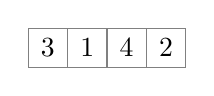
\begin{tikzpicture}
	\draw[step=0.5cm,color=gray] (-1,-1) grid (1,-0.5);
	\node at (-0.75,-0.75) {3};
	\node at (-0.25,-0.75) {1};
	\node at (0.25,-0.75) {4};
	\node at (0.75,-0.75) {2};
\end{tikzpicture}
\end{center}
 encodes the solution in which job $1$, belonging to class $A$, is scheduled in second position, while jobs $2$, $3$ and $4$, belonging to class $B$, are scheduled in fourth, first, and third position, respectively. Then, following the new notation, we have $[1]=3$, $[2]=1$, $[3]=4$, and $[4]=2$.\\
 Concerning with fitness evaluation, since individual with higher fitness are preferred by GAs but we are dealing with a minimization problem, we proceed as follows.\\Let $S$ be a solution for the BAWCT. We compute $f(S)$, i.e. its corresponding objective function value, by using \refe{BAWCT} and then we set $fitness_S = \frac{1}{f(S)}$.\\ In this way, when $f(S) \rightarrow 0 $ (that is a trivial lower bound for \refe{BAWCT}) follows that $fitness_S \rightarrow \infty$.
\subsection{Initial population}
Once the encoding strategy has been defined, the next step to be performed regards the generation of the initial population. A review of the main approaches used in this phase of GAs is done in \cite{init1}.\\
In our approach, we tried three different techniques: \textit{Random}, \textit{Alternated}, and \textit{Bidirectional}. Since the first strategy works randomly and we risk to create an initial population of completely unbalanced schedules, we defined the other two greedy techniques, in order to provide possibly the algorithm with a better starting point.\\
Let $N = \{1,\ldots,n_A+n_B\}$, $N_A =\{1,\ldots,n_A\}$, and $N_B=\{n_A+1,\ldots,n_A+n_B\}$. The three techniques we used can be formalized as follows:
\begin{itemize}
	\item \textit{Random generation}. The genotype of each individual is given by a random permutation of $N$ trivially representing a feasible solution for the BAWCT. Formally, let $P(N)$ be a random permutation of $N$, we set $[i] =  P(N)_i$. 
	\item \textit{Alternated generation}. The genotype of each individual is given by alternating jobs of the two classes, until one of the two sets is completely scheduled. Afterwards, potentially remaining jobs are accommodated at the end of the sequence.\\
	 Let $P(N_A)$ and $P(N_B)$ be two permutations of $N_A$ and $N_B$ respectively. The generation process can be formally summarized into two different phases:
	\begin{enumerate}
		\item Let $k = \min\{n_A,n_B\}$. In this phase $k$ steps are performed, each of which aimed at scheduling one job for each of the two classes. In particular, for $i=1,\ldots,k$, we set $[i] = P(N_A)_i$ and $[i+1] = P(N_B)_i$.
		\item This phase is performed whenever $n_A \ne n_B$. If this is the case, remaining jobs for one of the two classes are accommodated at the end of the sequence.\\ Assume $n_A<n_B$, then, for $i=k+1,\ldots,\max\{n_A,n_B\}$, we set $[k+i] = P(N_B)_i.$ If $n_A>n_B$, it's enough to substitute $P(N_B)$ with $P(N_A)$. 
	\end{enumerate}
	\item \textit{Bidirectional generation}. The genotype of each individual is given by scheduling, at each step of the process, one job for each of the two classes, inserting one of them in the first available position and the other in the last one. At each step, the choice among the two possible assignments is done in a greedy way.\\
	Let $P(N_A)$ and $P(N_B)$ be two permutations of $N_A$ and $N_B$, respectively. The generation process can be then formally summarized into two different phases:
	\begin{enumerate}
		\item Let $k = \min\{n_A,n_B\}$. In this phase $k$ steps are performed, each of which aimed at scheduling one job for each of the two classes.\\ In particular, for $i=1,\ldots,k$, we set either \be \label{eq1}[i] = P(N_A)_i \mbox{ and } [n_A+n_B-i] = P(N_B)_i\ee or \be \label{eq2}[i] = P(N_B)_i \mbox{ and } [n_A+n_B-i] = P(N_A)_i.\ee Following a greedy approach, among \refe{eq1} and \refe{eq2}, the assignment currently minimizing \refe{BAWCT} is chosen.  
		\item As for the previous technique, this phase is performed whenever $n_A \ne n_B$. If this is the case, remaining jobs for one of the two classes are now accommodated in the middle of the sequence. \\Assume $n_A<n_B$, then, for $i=k+1,\ldots,\max\{n_A,n_B\}$, we set $[i] = P(N_B)_i.$ If $n_A>n_B$, it's enough to substitute $P(N_B)$ with $P(N_A)$. 
	\end{enumerate}
	It's worth noting that in the \textit{Alternated} and \textit{Bidirectional generation}, for each different couple of permutations $(P(N_A),P(N_B))$, the generation process outputs a different schedule. This is crucial since it guarantees a \textit{diversification} in the initial population, even if the same greedy procedure is used for generating each individual.\\ It's trivial to see that this is the case even for the \textit{Random generation.}
\end{itemize}
\subsection{Selection}
Selection (see for example \cite{sel1}) is a crucial step in designing GAs since it defines the chance of a given individual to participate in the reproduction process. Since a convergence to optimal solutions is desired, it's recommended to give an higher chance to individuals having high fitness values.\\
In this work, we tested three different well-known selection techniques: \textit{Roulette wheel}, \textit{Binary tournment}, and \textit{k-tournment.}
\begin{itemize}
	\item \textit{Roulette wheel}. Following this technique, the selection is performed by simulating a roulette wheel in which each individual has a chance to be selected for reproduction represented by a portion of the roulette. Since the size of this portion depends on its fitness value, each individual $I$ has a probability $p_I$ to be selected that is directly proportional to its fitness.\\In particular, letting $P$ be the population of individuals, we set $$p_I = \frac{fitness_I}{\ds\sum_{i \in P}fitness_i}.$$
	\item \textit{Binary tournament}. From two randomly selected individuals, the one having highest fitness value is chosen for reproduction.
	\item \textit{k-tournament}. It's the same as the previous with the only difference that $k$ individuals are involved in the tournament. 
\end{itemize}
\subsection{Crossover}
Once parents are selected, they have to reproduce in order to generate new children. The reproduction process is simulated using crossover operators, aimed at creating a new individual whose features depend on both the parents by mixing their genetic properties. From an algorithmic point of view, this phase is crucial since it allows to navigate the solution space. \\
In literature a lot of crossover operators were proposed for scheduling problems and, in general, for sequencing problems like the well-known traveling salesman problem (for a general overview see \cite{cross1}). However, in \cite{sched1}, the authors noticed that crossover operators mainly proposed for traveling salesman problems don't perform very well in a scheduling context. Then, on the basis of their results, we implemented the following crossover operators: \textit{One-point crossover}, \textit{Two-point crossover Ver. I}, \textit{Two-point crossover Ver. II}, \textit{Position based crossover}, and, additionally, we defined a new crossover operator named \textit{k-AlternateCrossover.} (which it turned out to be very effective o eventualmente toglierlo(?)) (inserire figure?)\\
Given two parents $I_1$ and $I_2$, the previous crossover operators can be described as follows: 
\begin{itemize}
	\item \textit{One-point crossover.} One point $i \in [1,n_A+n_B]$ is randomly selected. Then, with the same probability, either the first $i$ jobs or the last $i$ ones are inherited from $I_1$, while the remaining $n_A+n_B-i$ are inserted in the sequence preserving the order of appearance they have in $I_2$. 
	\item \textit{Two-point crossover Ver. I.} Two points $i,j \in [1,n_A+n_B]$ are randomly selected. Suppose $i \le j$, the first $i$ jobs and the last $n_A+n_B-j$ ones are inherited from $I_1$, while the remaining $j-i$, exactly as in one-point crossover, are inserted in the sequence preserving the order they have in $I_2$.
	\item \textit{Two-point crossover Ver. II.} Two points $i,j \in [1,n_A+n_B]$ are randomly selected. Suppose $i \le j$, from position $i$ to $j$ the jobs are inherited from $I_1$, while the remaining jobs, following the same policy of one-point crossover, are inserted preserving the order they have in $I_2$.
	\item \textit{Position based crossover.} First of all, a number of positions $k \in [1,n_A+n_B]$ is randomly selected, then $k$ different values $v_i$, $i=1,\ldots,k$, are sampled in the interval $[1,n_A+n_B].$ At this point the jobs in positions $v_i$, for $i=1,\ldots,k$, are inherited from $I_1$, while the others, following the same idea of one-point crossover, are inserted preserving the order they have in $I_2$.
	\item \textit{Batch crossover}
\end{itemize}
\subsection{Mutation}
Another important operator in GAs is mutation, strictly related to crossover since, even mutation, it allows to navigate the solution space. In particular, mutation operators perturb the current solution by applying random changes.
Inspired by \cite{sched1}, in this work we tested the following four mutation operators:
\begin{itemize}
	\item \textit{Adjacent two-job change.} A position $i \in [1,n_A+n_B-1]$ is randomly selected and jobs in position $i$ and $i+1$ are swapped.
	\item \textit{Arbitrary two-job change.} Two different positions $i,j \in [1,n_A+n_B]$ are randomly selected and jobs in position $i$ and $j$ are swapped.
	\item \textit{Arbitrary three-job change.} Three different positions $i,j,k \in [1,n_A+n_B]$ are randomly selected and the corresponding jobs are swapped by setting at the same time: $[j] = [i]$, $[k] = [j]$, and $[i] = [k]$. 
	\item \textit{Shift change.} Two different positions $i,j \in [1,n_A+n_B]$ are randomly selected and job in position $i$ is moved in position $j$ by shifting all the intermediate jobs.
\end{itemize} 
Additionaly, by considering a set of adjacent jobs as an (atomic) \textit{batch}, we defined other two mutation operators:
\begin{itemize}
	\item \textit{Adjacent batch change.} A position $i \in [1,n_A+n_B-1]$ and a batch size $s \in [1,\lfloor{\frac{n_A+n_B-i+1}{2}}\rfloor]$ are randomly selected. Then, for $k=0,\ldots,s-1$, jobs in position $i+k$ and $i+s+k$ are swapped.
	\item \textit{Arbitrary batch change.} Two positions $i,j \in [1,n_A+n_B]$ are randomly selected. Suppose $i\le j$, also the batch size $s \in [1, \min\{j-i,n_A+n_B+1-j\}]$ is randomly determined. Then, for $k=0,\ldots,s-1$, jobs in position $i+k$ and $j+k$ are swapped. 
\end{itemize}
\subsection{Local Search}
As already specified in the introduction to our heuristics, in order to improve the fitness of new children, a local search (see for example \cite{local}) is applied immediately after mutation. The introduction of local search in our approach turned out to be very effective in practice since, in a lot of scenarios, starting from a "good" solution produced by the previous phases, it's able to reach an optimal one lying in the neighborhood.\\
In this work, as in [2], we implemented a 2-opt strategy first introduced in \cite{2-opt} for solving traveling salesman problems. In particular, given an individual $I$ representing a solution $S$, for each of the $\frac{(n_A+n_B)(n_A+n_B-1)}{2}$ couples of indices $(i,j)$, with $i<j$,  we check if by swapping jobs in position $i$ and $j$ we obtain a decrease in the current value of \refe{BAWCT}. If this is the case, we execute the exchange and we iterate the process.\\
It's worth to specify that, in order to evaluate the variation of \refe{BAWCT} for each possible exchange $(i,j)$, it's not necessary to compute afresh its value, since it can be done by a simple procedure iterating in the sequence from position $i$ to position $j$ (see [2]). Even if the overall worst-case complexity for computing the variation of \refe{BAWCT} is however linear ($\mathcal{O}(n_A+n_B)$) also in this case, avoid its recalculation has a not negligible impact on the overall performance.
\section{Numerical Results}
Scelta dei parametri, commento sull'utilità dell'inizializzazione intelligente con relativa tabella della fitness iniziale. 
\begin{table}[h]\scriptsize
	\begin{center}
		\begin{tabular}{|| c |c | c|| c||c ||}\hline
			
			\multirow{3}{*}{$n$} & \multirow{3}{*}{$n_A$} & \multirow{3}{*}{$n_B$} & \multirow{3}{*}{Exit(s)} & \multirow{3}{*}{Iter}\\
			&  &&  & \\
			&    &    &  &\\\hline
			$20$	 & \multirow{3}{*}{$10$}   & $10$   &$0,028$  & $19,1$
			\\
			$30$  &  & $20$	 & $0,017$
			&$6,4$
			\\ 
			$40$  &  & $30$	 & $0,028$
			&$5,6$
			\\ \hline
			
			$40$	 & \multirow{3}{*}{$20$}   & $20$   & $0,028$
			& $5,7$
			\\
			$50$  &  & $30$	 &$0,08$
			&$9,6$
			\\ 
			$60$  &  & $40$	 &$0,068$ &$3,7$\\ \hline
			
			$60$	 & \multirow{3}{*}{$30$}   & $30$   &  $0,067$
			& $3,6$
			\\
			$70$  &  & $40$	 &$0,19$
			&$7$
			\\ 
			$80$  &  & $50$	 & $0,32$
			&$7,7$
			\\ \hline
			
			$80$	 & \multirow{3}{*}{$40$}   & $40$   &  $0,091$
			&$2,2$
			\\
			$90$  &  & $50$	 & $0,748$
			&$11,6$
			\\ 
			$100$  &  & $60$	 & $0,347$
			&$4,4$
			\\ \hline 
		\end{tabular}
	\end{center}
	\caption{Small test problems, $p \in [1,25].$} \label{large}
\end{table}

\begin{table}[h]\scriptsize
	\begin{center}
		\begin{tabular}{|| c |c | c|| c||c ||}\hline
			
			\multirow{3}{*}{$n$} & \multirow{3}{*}{$n_A$} & \multirow{3}{*}{$n_B$} & \multirow{3}{*}{Exit (s)} & \multirow{3}{*}{Iter}\\
			&  &&  & \\
			&    &    &  &\\\hline
			$100$	 & \multirow{2}{*}{$50$}   & $50$   & $0,416$
			&$5,5$
			\\
			$150$  &  & $100$	 &$0,863$
			&$3,6$
			\\ \hline
			
			$200$	 & \multirow{2}{*}{$100$}   & $100$   & $1,705$
			&$2,8$
			\\
			$250$  &  & $150$	 & $6,121$
			&$4,4$
			\\ \hline
			
		\end{tabular}
	\end{center}
	\caption{Medium test problems, $p \in [1,50].$} \label{large}
\end{table}


\begin{table}[h]\scriptsize
	\begin{center}
		\begin{tabular}{|| c |c | c|| c||c ||}\hline
			
			\multirow{3}{*}{$n$} & \multirow{3}{*}{$n_A$} & \multirow{3}{*}{$n_B$} & \multirow{3}{*}{Exit (s)} & \multirow{3}{*}{Iter}\\
			&  &&  & \\
			&    &    & &\\\hline
			$300$	 & \multirow{2}{*}{$150$}   & $150$   &$14,566$
			& $5,3$
			\\
			$350$  &  & $200$	 &$ 62,988$
			&$11,7$
			\\ \hline
			
			$400$	 & \multirow{2}{*}{$200$}   & $200$   &$ 24,737$
			&$3,2$
			\\
			$450$  &  & $250$	 &$135,138$
			&$11,3$
			\\ \hline
			
			$500$	 & $250$   & $250$   &  $49,91$
			&$2,8$
			\\ \hline
			
		\end{tabular}
	\end{center}
	\caption{Large test problems, $p \in [1,100].$} \label{large}
\end{table}


\begin{table*}[h]\scriptsize
	\begin{center}
		\begin{tabular}{||c| c |c | c|| c||c ||c|| c||}\hline
			\multirow{3}{*}{$p \in [1,3n]$} &\multirow{3}{*}{$n$} & \multirow{3}{*}{$n_A$} & \multirow{3}{*}{$n_B$} & \multirow{2}{*}{Time for } & \multirow{3}{*}{Iter}& \multirow{2}{*}{Absolute Error }& \multirow{3}{*}{Solved to Opt}\\
			& &  &&  && & \\
			& &  &&Incumbent (s)  &&(\%)& \\
			
			\hline
			$p\in[1,180]$	 & $60$ & $30$   & $30$   &  1,83
			&  119,8 &0&20/20
			\\
			
			$p\in[1,300]$	 & $100$ & $50$   & $50$   &  6,207
			& 81,9&0&20/20
			\\
			$p\in[1,600]$ &$200$  &  $100$	 & $100$ &202,428
			&322,5&0&20/20
			\\ 
			
			$p\in[1,900] $ & $300$	 & $150$   & $150$   & 782,097
			& 339,4 &0,002 & 16/20
			
			\\
			$p\in[1,1200]$ & $400$  & $200$	 & $200$ & 1087,752
			&183 &0,004&11/20
			
			\\ 
			
			$p\in[1,1500]$ & $500$	 & $250$   & $250$   & 960,657
			
			& 91,5
			&0,008 &2/20
			
			\\ \hline
			
		\end{tabular}
	\end{center}
	\caption{Test problems with large ranges} \label{large}
\end{table*}




\section{Conclusions}



\bibliographystyle{informs2014} 
\bibliography{sched}


\end{document}

